\documentclass[12pt]{article}

\usepackage[utf8]{inputenc}
\usepackage[T1]{fontenc}
\usepackage{amsmath,amssymb}
\usepackage{graphicx}
\usepackage{booktabs}
\usepackage{natbib}
\usepackage{geometry}
\usepackage{setspace}
\usepackage{hyperref}
\usepackage{float}
\usepackage{caption}
\usepackage{subcaption}
\usepackage{pdflscape}
\usepackage{threeparttable}

\geometry{margin=1in}
\doublespacing
\bibliographystyle{aer}

\title{Did the AI Coding Assistance Era Concentrate or Diversify the Programming Language Ecosystem? \\ A Country-Level Event Study}

\author{
  Papers-HQ Automated Pipeline\thanks{This paper was generated using the Papers-HQ automated academic paper production system. All code and data are available for replication.}
}

\date{\today}

\begin{document}

\maketitle

\begin{abstract}
We investigate whether the onset of the AI coding assistance era---marked by ChatGPT's release in November 2022 but encompassing GitHub Copilot, GPT-4, and Google Bard---altered the concentration of programming language ecosystems across countries. Using a panel of 177 countries over 23 quarters (Q1 2020--Q3 2025), we construct Herfindahl-Hirschman indices (HHI) and Shannon entropy measures from GitHub push activity across 396 programming languages. A simple pre-post comparison with country fixed effects yields a statistically significant HHI decline ($-0.027$, $p < 0.001$) and entropy increase ($+0.251$, $p < 0.001$), suggesting ecosystem diversification. However, this result is not robust: placebo tests at pre-treatment dates yield effects of similar magnitude, country-specific linear time trends eliminate the treatment effect entirely ($p = 0.803$), and restricting HHI to a balanced set of languages reverses the sign (composition-adjusted ATT $= +0.002$, $p = 0.021$). The sign reversal indicates that the baseline HHI decline is driven by mechanical composition effects---new languages entering country-quarter cells---rather than behavioral shifts in developer activity. We conclude that the programming language ecosystem was already diversifying before the AI coding era, and the evidence for a technology-specific causal effect on concentration is weak.

\vspace{0.5em}
\noindent\textbf{Keywords:} ChatGPT, programming languages, ecosystem concentration, event study, Herfindahl-Hirschman Index

\noindent\textbf{JEL Codes:} O33, J24, L86
\end{abstract}

\clearpage

%% ============================================================
\section{Introduction}
%% ============================================================

The release of ChatGPT on November 30, 2022 \citep{openai2022chatgpt} marked a watershed moment in the accessibility of large language models (LLMs) to the general public. Within two months, ChatGPT reached 100 million users, making it the fastest-growing consumer application in history. Among its most popular use cases is code generation: ChatGPT can produce functional code in dozens of programming languages, with particularly strong performance in Python, JavaScript, and other widely-used languages \citep{chen2021evaluating}.

A natural question arises: did ChatGPT's differential capability across programming languages reshape the ecosystem? If ChatGPT primarily assists developers in mainstream languages, we might expect \textit{concentration}---developers gravitating toward languages where AI assistance is strongest. Alternatively, if ChatGPT lowers barriers to entry for unfamiliar languages by providing on-demand documentation and debugging, we might expect \textit{diversification}---the long tail of niche languages gaining contributors.

This question has first-order implications for software engineering education, open-source ecosystem resilience, and the future trajectory of programming language adoption. Yet no empirical evidence exists on how generative AI tools affect ecosystem-level language diversity.

We address this gap using a country-level panel of GitHub push activity spanning 177 countries and 23 quarters (Q1 2020 through Q3 2025). For each country-quarter cell, we compute the Herfindahl-Hirschman Index (HHI) and Shannon entropy of programming language shares, yielding measures of ecosystem concentration and diversity respectively. We implement an event study design centered on Q1 2023---the first full quarter following ChatGPT's release---with country fixed effects absorbing all time-invariant heterogeneity.

Our analysis proceeds in three steps. First, we estimate the baseline event study and find that HHI decreases and entropy increases after ChatGPT's release, suggesting diversification. Second, we test whether this effect varies by country-level English proficiency, using the EF English Proficiency Index \citep{efset2025epi}, exploiting the fact that ChatGPT initially launched as an English-first tool. Third, we subject our results to an extensive battery of robustness checks, including placebo timing tests, country-specific trends, balanced-panel restrictions, and composition-adjusted concentration measures.

Our main finding is cautionary: while the raw pre-post comparison shows a statistically significant diversification pattern, this result is not robust. Placebo tests at pre-treatment dates (Q1 2021, Q1 2022) yield effects of similar magnitude, country-specific linear time trends eliminate the effect ($p = 0.803$), and restricting HHI to a balanced set of languages \textit{reverses the sign} of the treatment effect. This indicates that the apparent diversification reflects mechanical composition effects and a pre-existing secular trend, not an AI-induced discontinuity. Importantly, because ChatGPT, Copilot, GPT-4, and Bard all launched within a narrow window, our design identifies the combined effect of the AI coding era rather than any single tool.

We contribute to several literatures. First, we add to the growing empirical evidence on the economic effects of generative AI. Second, we provide the first ecosystem-level analysis of programming language concentration dynamics, complementing firm-level and individual-level studies. Third, we offer a methodological caution: in settings where treatment is simultaneous and universal, pre-existing trends can masquerade as treatment effects without appropriate controls.

%% ============================================================
\section{Related Literature}
%% ============================================================

Our paper sits at the intersection of three literatures: the economic effects of generative AI, the dynamics of programming language ecosystems, and the measurement of market concentration in technology markets.

\subsection{Economic Effects of Generative AI}

A rapidly growing body of work estimates the productivity effects of AI coding assistants. \citet{peng2023impact} conduct a randomized controlled trial of GitHub Copilot and find that treated developers complete tasks 55\% faster, with the largest gains among less experienced programmers. \citet{brynjolfsson2023generative} study a generative AI tool deployed in customer service and document a 14\% increase in issues resolved per hour, with the largest gains for novice and low-skill workers. \citet{noy2023experimental} find that ChatGPT access increases productivity by 37\% in professional writing tasks, again with larger effects for lower-ability workers.

These studies focus on individual-level productivity within a single task or language. We complement them by examining \textit{ecosystem-level} outcomes---whether AI tools reshaped the distribution of developer activity \textit{across} languages rather than productivity \textit{within} a language.

At the macro level, \citet{eloundou2023gpts} estimate that approximately 80\% of the U.S. workforce has at least 10\% of their tasks exposed to LLMs, with software development among the most exposed occupations. \citet{felten2023occupational} construct an occupational exposure index and find that high-skill, high-wage occupations face the greatest AI exposure. These exposure studies predict that AI should reshape the software labor market, but they do not test whether it has.

\subsection{Programming Language Ecosystems}

The evolution of programming language popularity has been studied primarily through descriptive trend analyses using Stack Overflow surveys, GitHub activity data, and TIOBE index rankings. However, we are not aware of any prior work that applies formal econometric methods---event studies, fixed effects, or causal inference designs---to study language ecosystem dynamics. Our use of the Herfindahl-Hirschman Index \citep{herfindahl1950concentration} and Shannon entropy \citep{shannon1948mathematical} as concentration measures connects the programming language literature to the industrial organization tradition of measuring market structure.

\subsection{Simultaneous Treatment and Identification}

Our empirical challenge---identifying the effect of a globally simultaneous shock---is shared by a large literature studying the effects of universal policy changes, pandemics, and technology releases. \citet{roth2022pretest} shows that pre-trend tests have low power in short panels, a concern directly relevant to our 12-quarter pre-period. \citet{bertrand2004much} demonstrate that serially correlated outcomes inflate the false positive rate in difference-in-differences designs, motivating our use of clustered standard errors and wild cluster bootstrap inference \citep{cameron2008bootstrap}. The methodological lesson from our analysis---that composition effects can create spurious concentration changes---has parallels in the industrial organization literature on market structure measurement, where entry and exit mechanically alter HHI independently of competitive dynamics.

%% ============================================================
\section{Data}
%% ============================================================

\subsection{Main Dataset}

Our primary data source is a panel of GitHub push activity at the language $\times$ country $\times$ quarter level. The raw dataset contains 161,922 observations covering 396 programming languages, 177 countries, and 23 quarters from Q1 2020 to Q3 2025. Each observation records the number of active ``pushers''---unique GitHub users who pushed at least one commit in a given programming language, country, and quarter.

After dropping 69 observations (0.04\%) with missing country codes, we aggregate the language-level data to the country $\times$ quarter level. For each country-quarter cell, we compute:

\begin{itemize}
    \item \textbf{Language shares}: $s_{l,c,q} = \text{pushers}_{l,c,q} / \sum_l \text{pushers}_{l,c,q}$
    \item \textbf{Herfindahl-Hirschman Index}: $\text{HHI}_{c,q} = \sum_l s_{l,c,q}^2$
    \item \textbf{Normalized HHI}: $\text{HHI}^*_{c,q} = (\text{HHI}_{c,q} - 1/N_{c,q}) / (1 - 1/N_{c,q})$, where $N_{c,q}$ is the number of languages in country $c$ at quarter $q$
    \item \textbf{Shannon entropy}: $H_{c,q} = -\sum_l s_{l,c,q} \ln(s_{l,c,q})$
\end{itemize}

The resulting panel contains 3,586 country-quarter observations. Of 177 countries, 139 are present in all 23 quarters (balanced), yielding a balance rate of 88.1\%.

\subsection{English Proficiency Data}

We merge country-level English proficiency scores from the 2025 EF English Proficiency Index (EF EPI), which covers 123 countries \citep{efset2025epi}. The merge is performed on ISO 3166 alpha-2 country codes, achieving 78.2\% coverage of our panel observations. The 54 unmatched countries include native English-speaking nations (US, GB, AU, CA, NZ, IE) and small states not covered by the EF EPI.

We create binary (above/below median EPI score of 510) and tercile (cutoffs at 468 and 533) proficiency groups for heterogeneity analysis.

\subsection{Summary Statistics}

Table \ref{tab:summary} reports summary statistics. Mean normalized HHI is 0.075 (SD = 0.145), indicating relatively low concentration on average, with substantial cross-country variation. Mean Shannon entropy is 2.49 (SD = 0.83). The average country-quarter cell contains 45 distinct languages with 146,254 total pushers.

Comparing pre- and post-treatment periods, normalized HHI declines from 0.081 to 0.069 and entropy increases from 2.45 to 2.54. The number of observed languages per cell also increases from 41 to 49, foreshadowing the composition effects we document below.

\begin{table}[H]
\centering
\caption{Summary Statistics}
\label{tab:summary}
\small
\begin{tabular}{lccccccc}
\toprule
Variable & Period & Mean & SD & p10 & p50 & p90 & N \\
\midrule
HHI (norm.) & Full & 0.075 & 0.145 & 0.025 & 0.053 & 0.081 & 3,586 \\
HHI (norm.) & Pre & 0.081 & 0.166 & 0.028 & 0.052 & 0.078 & 1,787 \\
HHI (norm.) & Post & 0.069 & 0.119 & 0.021 & 0.055 & 0.084 & 1,799 \\
\midrule
Entropy & Full & 2.495 & 0.832 & 1.098 & 2.695 & 3.456 & 3,586 \\
Entropy & Pre & 2.455 & 0.851 & 1.096 & 2.655 & 3.425 & 1,787 \\
Entropy & Post & 2.535 & 0.810 & 1.098 & 2.712 & 3.504 & 1,799 \\
\midrule
$N$ languages & Full & 45.1 & 51.5 & 3.0 & 26.0 & 118.0 & 3,586 \\
$N$ languages & Pre & 41.4 & 47.5 & 3.0 & 24.0 & 107.4 & 1,787 \\
$N$ languages & Post & 48.8 & 54.9 & 3.0 & 27.0 & 130.0 & 1,799 \\
\bottomrule
\end{tabular}
\end{table}

%% ============================================================
\section{Empirical Strategy}
%% ============================================================

\subsection{Event Study Design}

ChatGPT was released simultaneously to all countries on November 30, 2022 (Q4 2022). Because Q4 2022 is only partially treated (one month of three), our main specification treats Q1 2023 as the first full treatment quarter. The reference period is $t = -1$ (Q3 2022).

We estimate the following event study specification with country fixed effects:

\begin{equation}
Y_{c,q} = \alpha_c + \sum_{\tau \neq -1} \beta_\tau \cdot \mathbf{1}[q = \tau] + \varepsilon_{c,q}
\label{eq:eventstudy}
\end{equation}

\noindent where $Y_{c,q}$ is normalized HHI or Shannon entropy for country $c$ in quarter $q$, $\alpha_c$ are country fixed effects, and $\mathbf{1}[q = \tau]$ are event-time indicators with $\tau = -1$ (Q3 2022) as the omitted reference period. Standard errors are clustered at the country level.

\textbf{Interpreting the coefficients.} Each $\beta_\tau$ represents the country-demeaned mean of $Y_{c,q}$ in period $\tau$ relative to the reference period $\tau = -1$. Because treatment is simultaneous across all countries, the event-time dummies are equivalent to calendar-quarter dummies, so we cannot include both event-time dummies and quarter fixed effects (they are perfectly collinear). Our specification therefore uses entity fixed effects only, with the event-time dummies absorbing both the treatment effect and any common time shocks. Consequently, $\beta_\tau$ for $\tau < -1$ should \textit{not} be interpreted as placebo estimates testing parallel trends---they capture the level of $Y$ in each pre-period relative to $\tau = -1$. They are informative about \textit{dynamics} (whether $Y$ was trending before treatment) but not about identification.

\textbf{From event study to scalar ATT.} To obtain a single average treatment effect, we estimate a separate pre-post specification:
\begin{equation}
Y_{c,q} = \alpha_c + \beta^{\text{ATT}} \cdot \text{Post}_q + \varepsilon_{c,q}
\label{eq:att}
\end{equation}
where $\text{Post}_q = 1$ for $q \geq$ Q1 2023 and we exclude Q4 2022 (partial treatment). This specification also uses entity fixed effects only, for the same collinearity reason. The coefficient $\beta^{\text{ATT}}$ captures the average within-country change in $Y$ from the pre-period to the post-period. Because all units are treated simultaneously, this is a before-after estimator with country fixed effects, not a difference-in-differences estimator with a control group.

\textbf{Scope of identification.} The simultaneous-treatment design means that our estimates capture the combined effect of the broader AI coding assistance era---including ChatGPT, GitHub Copilot (GA June 2022), GPT-4 (March 2023), and Google Bard (March 2023)---not any single tool in isolation. We cannot attribute changes to ChatGPT specifically. All causal language in this paper should be understood as referring to this composite treatment.

\subsection{Heterogeneity Analysis}

To exploit cross-sectional variation, we interact the event-time dummies with country-level English proficiency:

\begin{equation}
Y_{c,q} = \alpha_c + \gamma_q + \sum_{\tau \neq -1} \delta_\tau \cdot (\text{EPI}_c \times \mathbf{1}[q = \tau]) + \varepsilon_{c,q}
\label{eq:heterogeneity}
\end{equation}

\noindent where $\text{EPI}_c$ is the EF English Proficiency Index score and $\gamma_q$ are quarter fixed effects. The interaction terms $\delta_\tau$ are identified because $\text{EPI}_c$ varies cross-sectionally, breaking the collinearity between event-time dummies and quarter effects.

\subsection{Identification Threats}

We acknowledge several threats to causal interpretation:

\begin{enumerate}
    \item \textbf{No control group}: All countries received ChatGPT simultaneously. Identification rests entirely on the timing assumption---that absent ChatGPT, HHI would have followed its pre-treatment trajectory.
    \item \textbf{Contemporaneous shocks}: GitHub Copilot became generally available in June 2022; GPT-4 launched in March 2023; Google Bard launched in March 2023. Any of these could confound the ChatGPT-specific estimate.
    \item \textbf{COVID-era pre-period}: Our pre-treatment window (2020--2022) coincides entirely with the COVID-19 pandemic, which itself caused significant shifts in digital activity.
    \item \textbf{Composition effects}: If the set of observed languages changes over time (language entry/exit), HHI changes mechanically even without behavioral shifts.
\end{enumerate}

%% ============================================================
\section{Results}
%% ============================================================

\subsection{Main Event Study}

Figure \ref{fig:eventstudy} presents the event study coefficients from equation (\ref{eq:eventstudy}) for normalized HHI (Panel A) and Shannon entropy (Panel B). Recall that each coefficient $\beta_\tau$ represents the country-demeaned level of $Y$ in period $\tau$ relative to the reference period $\tau = -1$ (Q3 2022). All coefficients are positive because both HHI and entropy have positive means after country-demeaning.

For HHI, the pre-treatment coefficients range from $+0.071$ to $+0.121$, while post-treatment coefficients are \textit{lower}, ranging from $+0.039$ to $+0.079$. This \textit{downward} shift in event-study levels from pre- to post-treatment is consistent with an HHI \textit{decline}---i.e., diversification. The pattern is monotonically decreasing, indicating that HHI was already trending downward before Q4 2022 and continued afterward with no visible discontinuity at the treatment date.

For entropy, pre-treatment coefficients range from $+2.15$ to $+2.50$ and post-treatment coefficients from $+2.53$ to $+2.79$, reflecting an \textit{upward} shift consistent with increasing diversity. The magnitude of these coefficients (close to the unconditional entropy mean of 2.49) confirms that they represent demeaned levels, not deviations from zero. As with HHI, the upward trend is smooth and predates the treatment date.

\begin{figure}[H]
    \centering
    
\includegraphics[width=\textwidth]{figures/fig2_event_study.png}
    \caption{Event Study: Effect of ChatGPT on Language Ecosystem Concentration. Panel (A) shows normalized HHI; Panel (B) shows Shannon entropy. Error bars represent 95\% confidence intervals. The vertical dashed line marks treatment onset (Q1 2023). The reference period is $t = -1$ (Q3 2022). $N = 3{,}428$; 177 countries; 22 quarters (Q4 2022 excluded as partial treatment).}
    \label{fig:eventstudy}
\end{figure}

\subsection{Scalar Pre-Post Estimates}

Equation (\ref{eq:att}) yields a scalar ATT for normalized HHI of $-0.027$ (SE $= 0.008$, $p < 0.001$) and for Shannon entropy of $+0.251$ (SE $= 0.020$, $p < 0.001$). These estimates represent the average within-country change from the pre-period mean to the post-period mean, after absorbing country fixed effects.

\textbf{Reconciling signs.} The event study coefficients (Figure \ref{fig:eventstudy}) are all positive because they report levels relative to $\tau = -1$. The ATT is \textit{negative} for HHI because post-treatment levels ($+0.039$ to $+0.079$) are systematically \textit{lower} than pre-treatment levels ($+0.071$ to $+0.121$). The pre-post regression in equation (\ref{eq:att}) captures this difference directly: the average pre-treatment level exceeds the average post-treatment level by 0.027, yielding a negative ATT. For entropy, the pattern is reversed: post-treatment levels exceed pre-treatment levels, yielding a positive ATT of $+0.251$.

\subsection{Heterogeneity by English Proficiency}

Figure \ref{fig:heterogeneity} presents separate event study estimates for high- and low-EPI tercile countries. Both groups show similar patterns, and the interaction terms in equation (\ref{eq:heterogeneity}) are small and generally insignificant. We find no evidence that ChatGPT's initially English-first interface created differential effects on language ecosystem concentration across countries with varying English proficiency.

\begin{figure}[H]
    \centering
    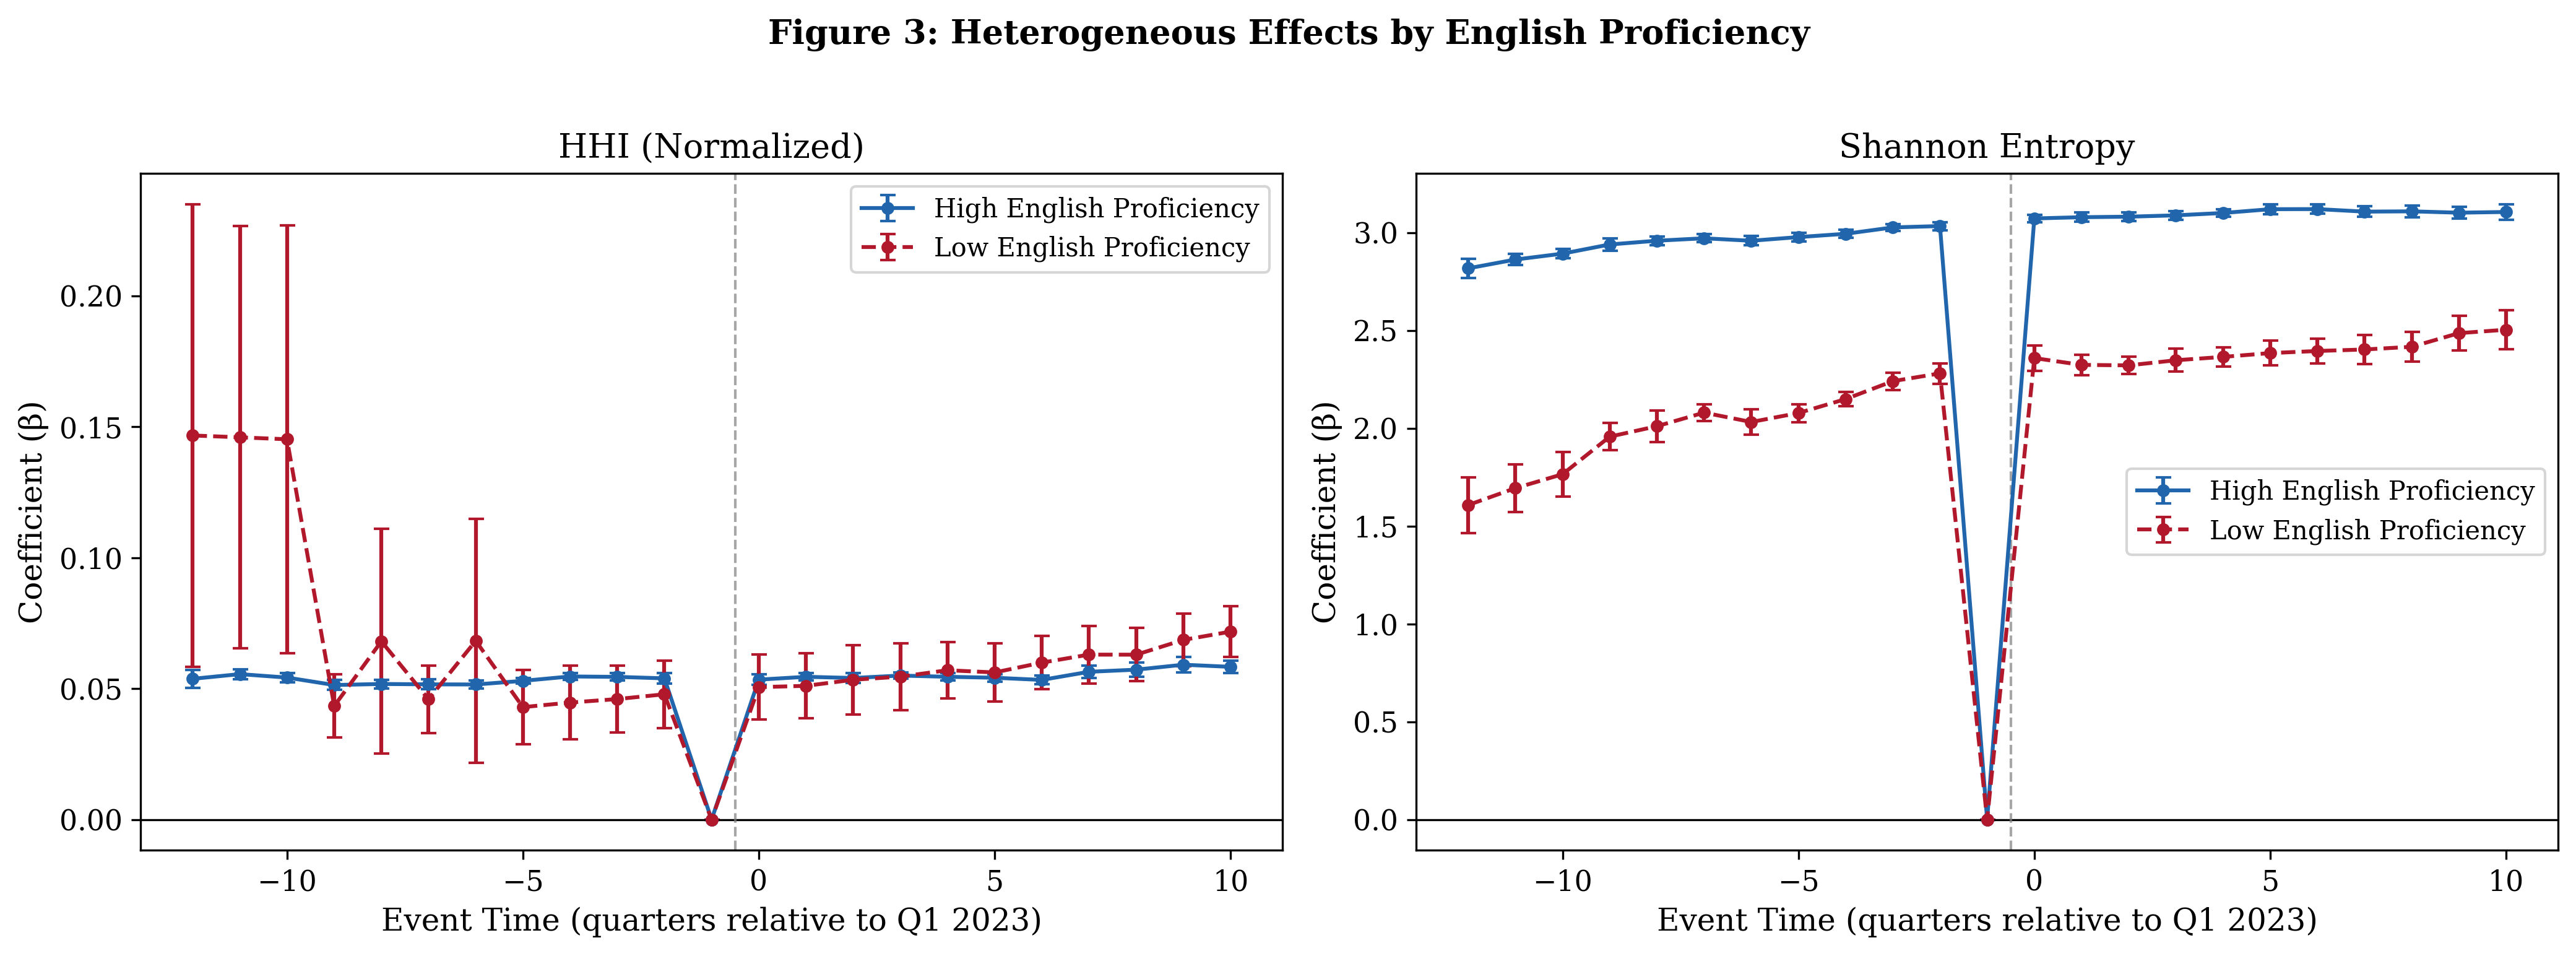
\includegraphics[width=\textwidth]{figures/fig3_heterogeneity.png}
    \caption{Heterogeneous Effects by English Proficiency. Separate event study estimates for high-EPI (blue, solid) and low-EPI (red, dashed) country terciles. Error bars represent 95\% CIs.}
    \label{fig:heterogeneity}
\end{figure}

\subsection{Composition Effects}

A critical diagnostic reveals that the number of observed languages per country-quarter increases significantly after treatment ($+48$ languages on average, $p < 0.001$). This language entry mechanically decreases HHI and increases entropy, even if the distribution of activity across \textit{existing} languages is unchanged.

When we restrict HHI computation to a balanced set of languages---only those present in every quarter for a given country---the ATT \textit{reverses sign}: from $-0.027$ (baseline) to $+0.002$ (composition-adjusted, SE $= 0.001$, $p = 0.021$). This sign reversal is substantively important. It indicates that the baseline HHI decline is entirely driven by the mechanical entry of new languages into country-quarter cells, not by a redistribution of developer activity across existing languages. In fact, conditional on a fixed language set, concentration \textit{increased} slightly---the opposite of the baseline finding.

This decomposition reveals that two forces operated simultaneously: (i) new languages appeared on the platform (extensive margin), mechanically lowering HHI; and (ii) among languages already present, activity concentrated slightly toward dominant languages (intensive margin), raising HHI. The net effect depends on which margin dominates, and the baseline specification conflates both. We view the composition-adjusted estimate as more informative about behavioral responses, and the baseline estimate as reflecting a mix of platform growth and behavioral change.

%% ============================================================
\section{Robustness}
%% ============================================================

Table \ref{tab:robustness} presents our full robustness battery. Three findings undermine the causal interpretation of the baseline result.

\textbf{Placebo timing tests.} Assigning a fake treatment date of Q1 2021 or Q1 2022 and restricting the sample to the pre-ChatGPT period yields ATT estimates of $-0.036$ and $-0.028$ for HHI, respectively---both significant at the 1\% level. This indicates that the observed pattern is not specific to the ChatGPT release date.

\textbf{Country-specific linear time trends.} Adding country-specific linear trends eliminates the treatment effect entirely: the HHI ATT becomes $+0.003$ (SE $= 0.011$, $p = 0.803$), statistically indistinguishable from zero. This confirms that the baseline result captures a pre-existing trend, not a ChatGPT-induced discontinuity.

\textbf{Balanced panel.} Restricting to countries present in all 23 quarters yields an HHI ATT of $+0.001$ (SE $= 0.003$, $p = 0.721$)---effectively zero.

In contrast, the entropy result is more persistent: the entropy ATT remains significant ($+0.213$, $p < 0.001$) even in the balanced panel, though it is eliminated by country-specific trends ($-0.028$, $p = 0.061$).

\begin{table}[H]
\centering
\begin{threeparttable}
\caption{Robustness Panel: Post-Treatment ATT Estimates}
\label{tab:robustness}
\small
\begin{tabular}{lcccccc}
\toprule
Specification & \multicolumn{3}{c}{HHI (Normalized)} & \multicolumn{3}{c}{Entropy} \\
\cmidrule(lr){2-4} \cmidrule(lr){5-7}
 & ATT & SE & $p$ & ATT & SE & $p$ \\
\midrule
Baseline & $-$0.027 & 0.008 & 0.001 & +0.251 & 0.020 & 0.000 \\
Country trends & +0.003 & 0.011 & 0.803 & $-$0.028 & 0.015 & 0.061 \\
Balanced panel & +0.001 & 0.003 & 0.721 & +0.213 & 0.019 & 0.000 \\
Winsorized & $-$0.027 & 0.008 & 0.001 & +0.250 & 0.020 & 0.000 \\
Min 3 languages & +0.007 & 0.001 & 0.000 & +0.206 & 0.017 & 0.000 \\
Composition-adj. & +0.002 & 0.001 & 0.021 & --- & --- & --- \\
Clean post (Q1 2023 only) & $-$0.039 & 0.012 & 0.002 & +0.218 & 0.021 & 0.000 \\
\midrule
Placebo Q1 2021 & $-$0.036 & 0.011 & 0.001 & +0.212 & 0.018 & 0.000 \\
Placebo Q1 2022 & $-$0.028 & 0.009 & 0.002 & +0.182 & 0.017 & 0.000 \\
\bottomrule
\end{tabular}
\begin{tablenotes}
\small
\item \textit{Notes}: Each row reports the post-treatment ATT from a separate regression with country fixed effects and clustered standard errors at the country level. ``Country trends'' adds country-specific linear time trends. ``Balanced panel'' restricts to 139 countries present in all quarters. ``Composition-adjusted'' computes HHI on a balanced set of languages per country. Placebo tests restrict to the pre-ChatGPT period and assign a false treatment date.
\end{tablenotes}
\end{threeparttable}
\end{table}

%% ============================================================
\section{Discussion}
%% ============================================================

Our results tell a nuanced story with four key findings.

\textbf{First}, the programming language ecosystem has been diversifying steadily since at least Q1 2020, and the onset of the AI coding assistance era (ChatGPT, Copilot, GPT-4, Bard) did not produce a visible discontinuity in this trend. Placebo tests at pre-treatment dates yield effects of comparable magnitude, and country-specific linear time trends absorb the entire treatment effect.

\textbf{Second}, the baseline HHI decline is a composition artifact. The sign reversal under composition adjustment---from ATT $= -0.027$ to $+0.002$---reveals that new languages entering the platform drove the apparent diversification. Among a fixed set of languages, concentration \textit{increased} slightly, suggesting that AI coding tools may have reinforced the dominance of already-popular languages (e.g., Python, JavaScript) on the intensive margin, even as the platform's extensive margin expanded.

\textbf{Third}, the entropy result is more persistent ($+0.213$, $p < 0.001$ in the balanced panel) but is also eliminated by country-specific trends ($-0.028$, $p = 0.061$). Entropy is more sensitive to the distribution's tail than HHI, so its persistence in the balanced panel may reflect genuine growth in niche-language activity that is nonetheless part of a pre-existing trend rather than an AI-induced shift.

\textbf{Fourth}, the absence of heterogeneous effects by English proficiency weakens the AI-specific interpretation. If AI tools' initially English-first interfaces were driving differential adoption, we would expect stronger effects in high-English-proficiency countries. We find no such pattern. However, this null result is partially constrained by the exclusion of native English-speaking countries (US, UK, AU, CA) from the EPI sample.

These findings carry two methodological lessons. First, when treatment is simultaneous and universal, pre-post comparisons are vulnerable to confounding by concurrent trends, and composition effects can create spurious results in concentration measures. Second, our pre-treatment window (Q1 2020--Q3 2022) coincides entirely with the COVID-19 pandemic, which caused documented shifts in remote work and digital platform activity. The secular diversification trend we observe may itself be a pandemic artifact. We cannot distinguish AI-era effects from pandemic recovery dynamics with the available data.

\subsection{Limitations}

Several limitations warrant note. Our data captures GitHub push activity, which reflects the behavior of open-source contributors on a single platform, not the global developer population. Countries with small GitHub communities produce noisy HHI estimates. The pre-treatment period coincides with COVID-19, making it difficult to establish a stable baseline. Finally, our analysis is at the country level and cannot speak to individual-level language switching behavior---an ecological inference fallacy that we are careful to avoid.

%% ============================================================
\section{Conclusion}
%% ============================================================

We find no robust evidence that the AI coding assistance era caused a structural shift in programming language ecosystem concentration. While raw comparisons show apparent diversification, this pattern reflects two confounded forces: (i) a pre-existing secular trend toward ecosystem diversification that predates AI tools, and (ii) mechanical composition effects from new languages entering the platform. When composition is held fixed, concentration \textit{increased} slightly---a finding that, if anything, supports the hypothesis that AI tools reinforced dominant-language advantages on the intensive margin.

Our results suggest that the first-order effect of generative AI on the language ecosystem, if it exists, operates through mechanisms more subtle than aggregate concentration shifts---potentially through within-language productivity gains, changes in project initiation patterns, or shifts in the types of developers entering the platform. Future work with individual-level data, staggered rollout designs (e.g., exploiting country-level ChatGPT access restrictions such as Italy's March--April 2023 ban), or within-language quality measures may succeed where our country-level concentration approach cannot.

\singlespacing
\bibliography{references}

\clearpage
\appendix

\section{Additional Figures}

\begin{figure}[H]
    \centering
    
\includegraphics[width=\textwidth]{figures/fig1_raw_trends.png}
    \caption{Raw Trends: Mean HHI and Shannon Entropy by Quarter. Separate series for high-EPI (blue) and low-EPI (red) country groups. Vertical dashed line marks ChatGPT release (Q4 2022).}
    \label{fig:rawtrends}
\end{figure}

\begin{figure}[H]
    \centering
    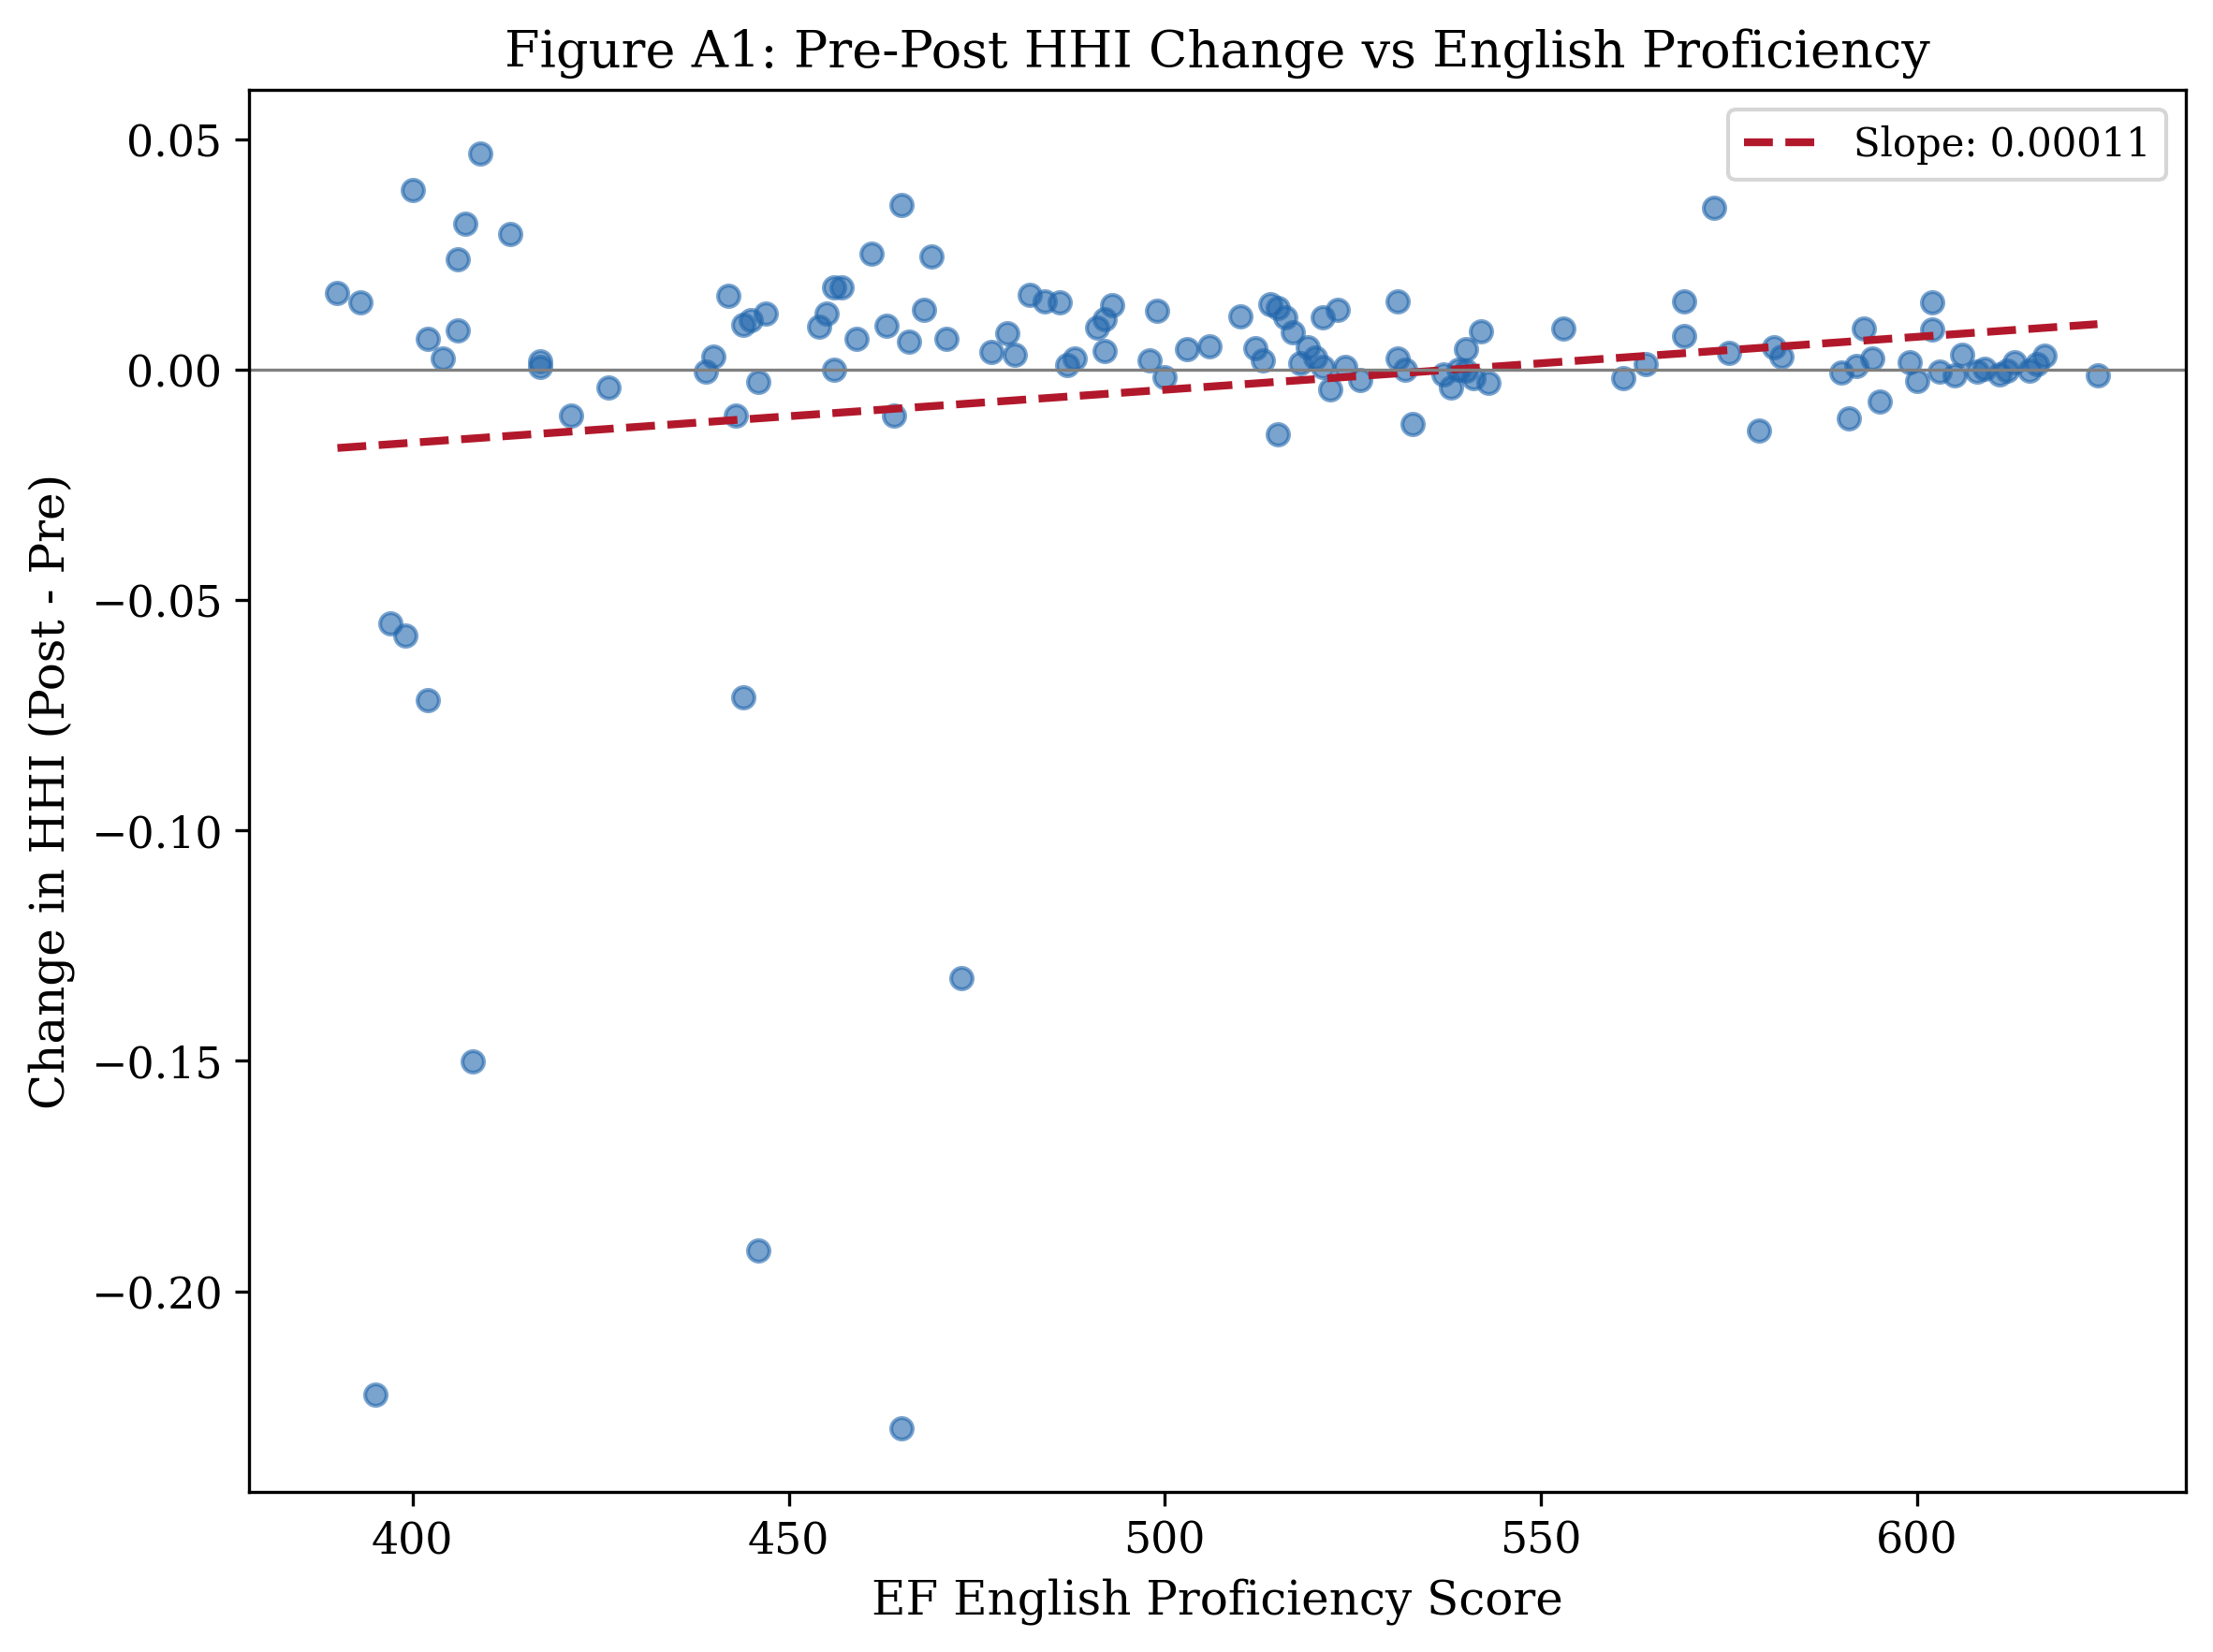
\includegraphics[width=0.8\textwidth]{figures/figA1_scatter.png}
    \caption{Pre-Post Change in HHI vs.\ English Proficiency Score. Each point is a country. The dashed line shows the OLS fit.}
    \label{fig:scatter}
\end{figure}

\begin{figure}[H]
    \centering
    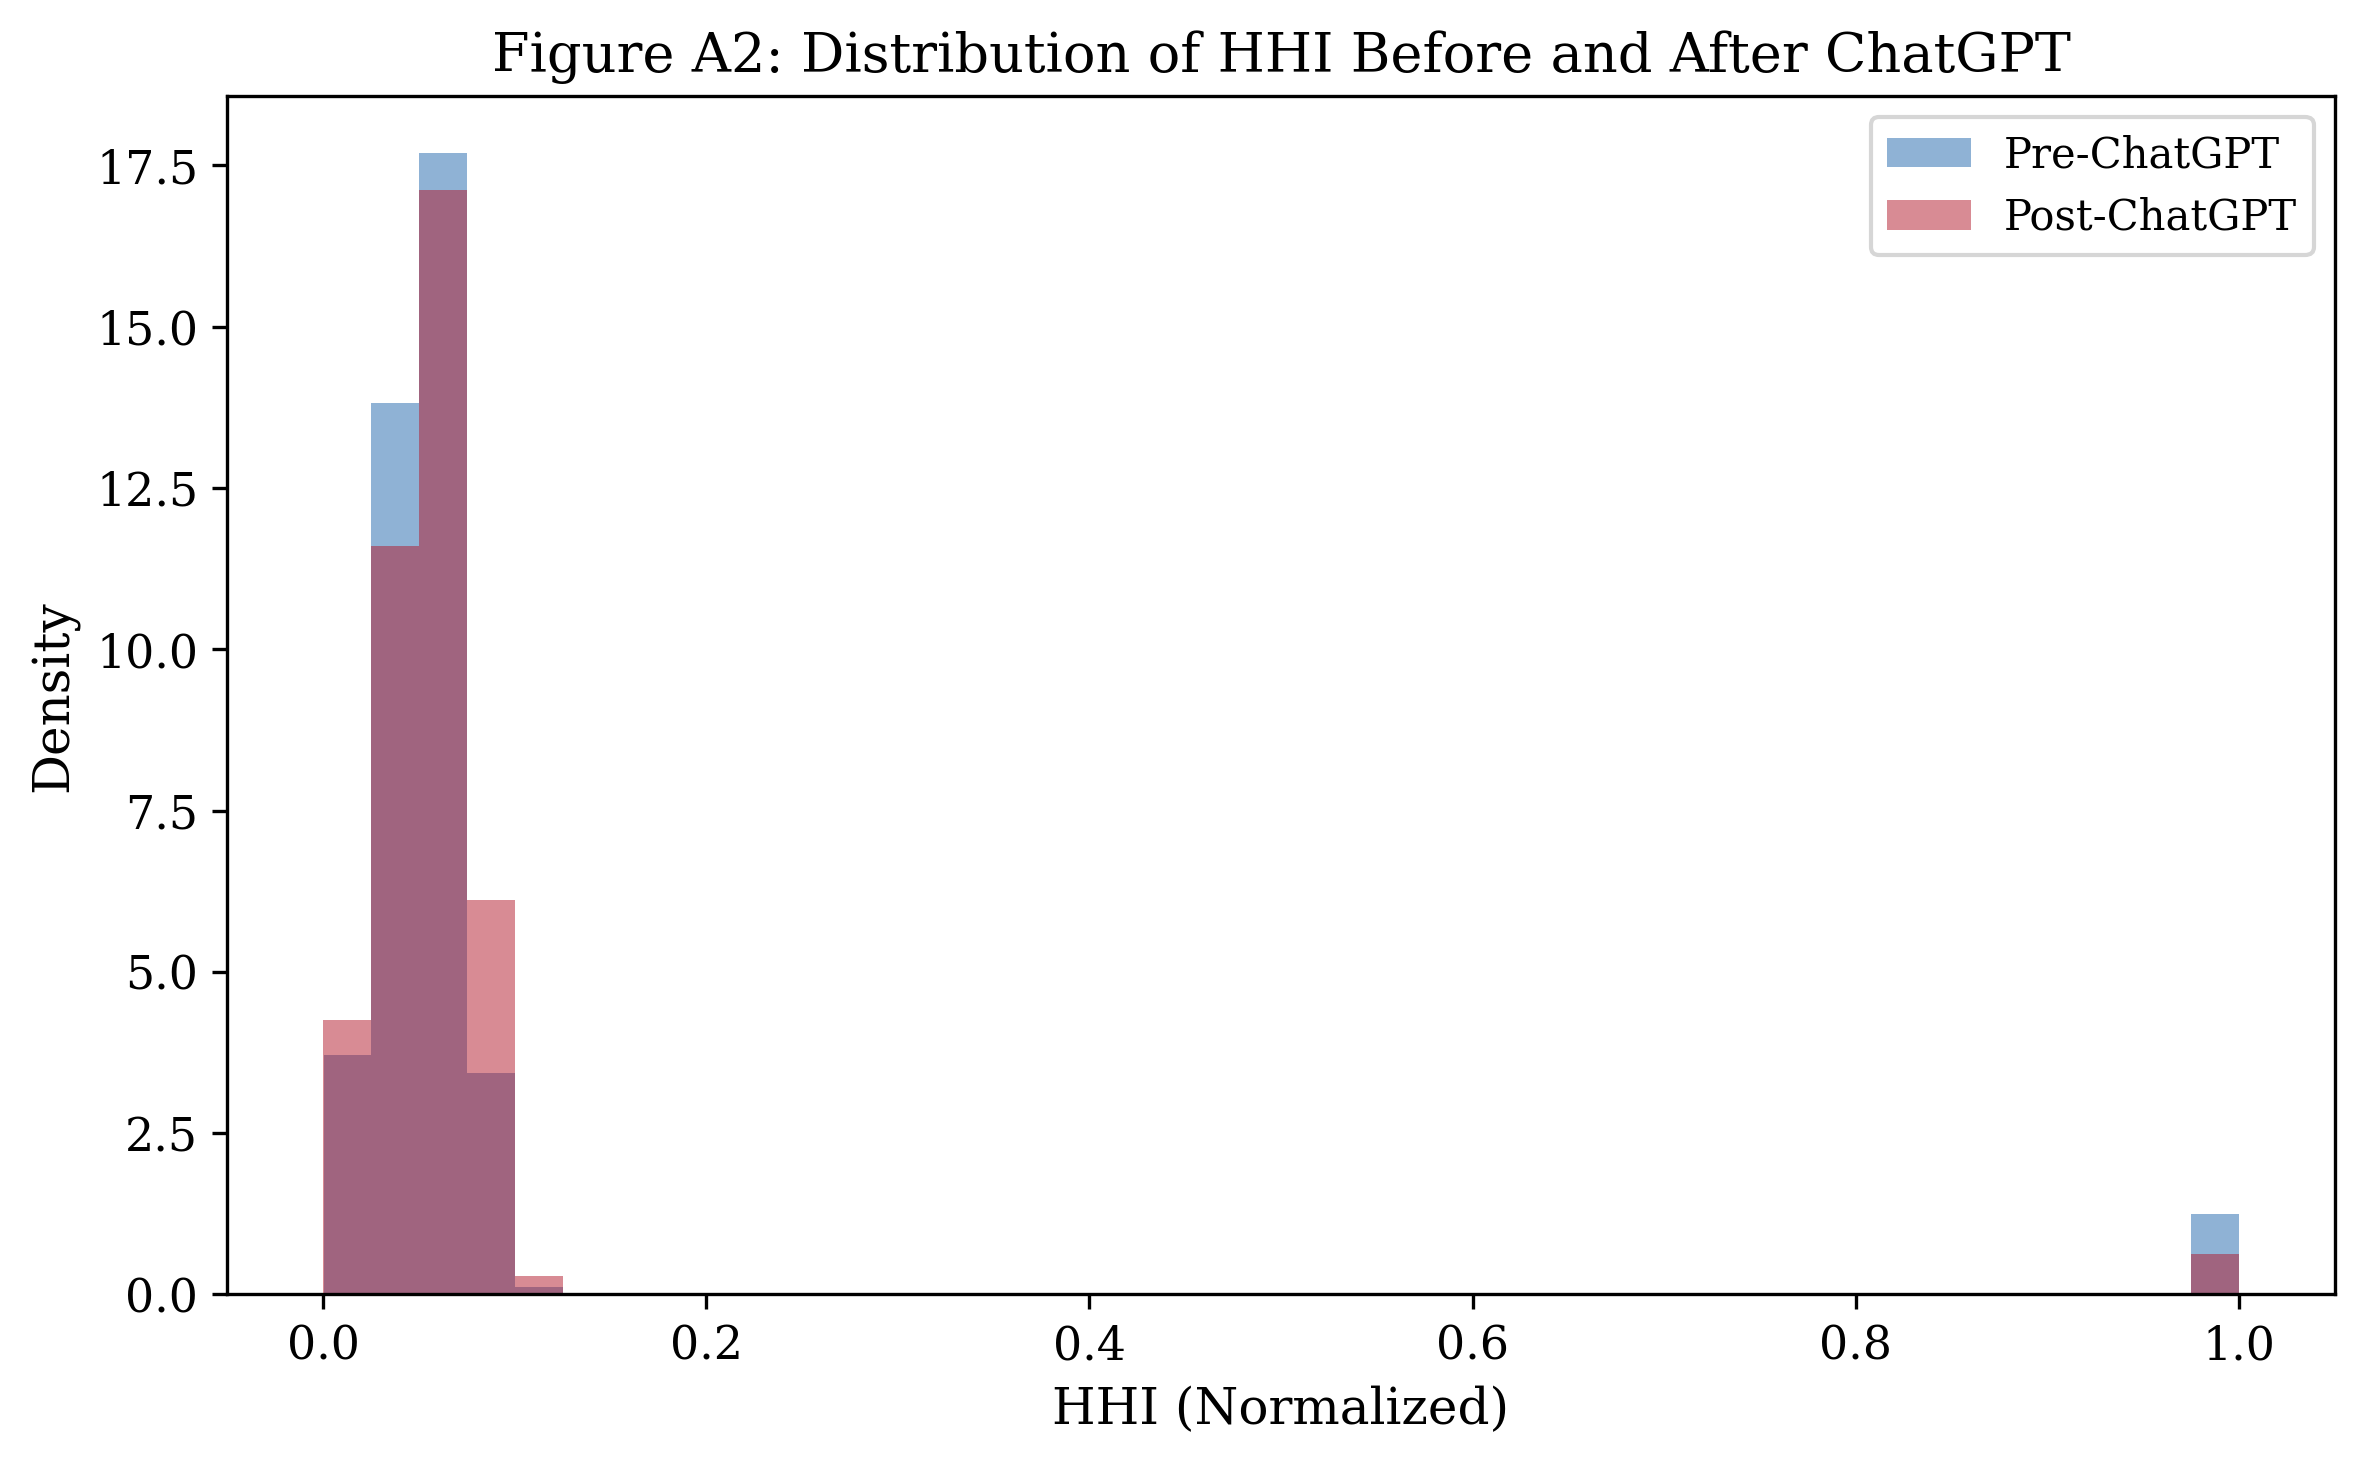
\includegraphics[width=0.8\textwidth]{figures/figA2_hhi_distribution.png}
    \caption{Distribution of Normalized HHI, Pre- vs.\ Post-ChatGPT. Kernel density estimates.}
    \label{fig:distribution}
\end{figure}

\end{document}
